\section{Representation of Failures in the Ontology}\label{task2}
A failure is any change or any design or manufacturing error that renders a component, assembly, or system incapable of performing its intended function. In kitting, failures can occur for multiple reasons: equipment not set up properly, tools and/or fixtures not properly prepared, lack of safety, and improper equipment maintenance. Part/component availability failures can be triggered by inaccurate information on the location of the part, part damage, wrong type of part, or part shortage due to delays in internal logistics. In order to prevent or minimize failures, a disciplined approach needs to be implemented to identify the different ways a process design can fail before impacting the productivity.

 Failures detected in the workstation can result in the current plan to become obsolete. When a failure is detected in the execution process and the failure mode identified, the value of the severity for the failure mode will be retrieved from the ontology and the appropriate contingency plan will be activated. In some cases, the current state of the environment is brought back to the state prior to the failure and the robot starts from a ``stable" state. To select the right contingency plan, i.e., the less time consuming or safer, the system will need to rely on the information from the knowledge representation.

In our kitting system, the \process{Predicate Evaluation} process is responsible for failure detection. An action failure consists of failure modes that can occur during the execution of a PDDL action. The steps to identify action failures in the kitting system are described in Figure~\ref{fig:algo}.

\begin{figure}[h!t!]
  \centering
  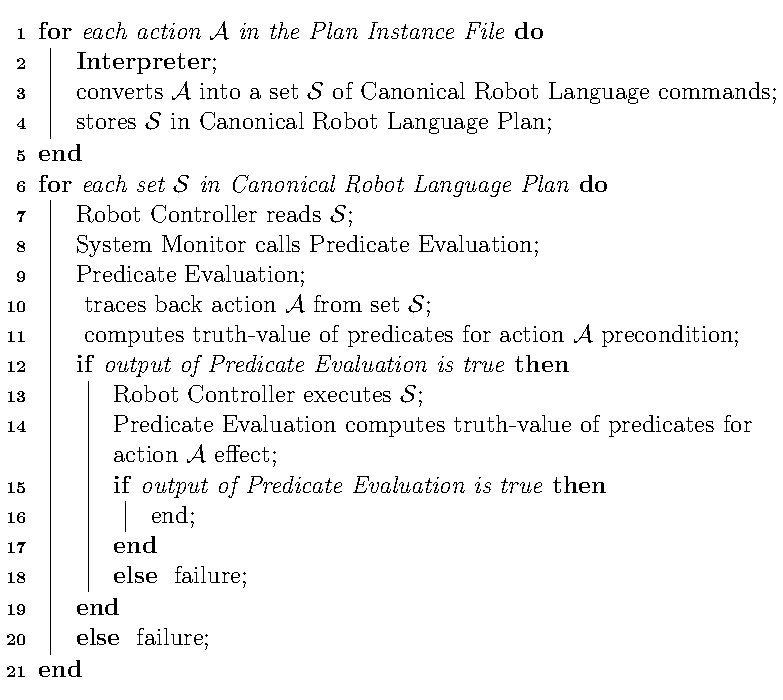
\includegraphics[width=9cm]{Figures/algorithm.pdf}
  \caption{Failure identification.}
  \label{fig:algo}
\end{figure}

As seen in Figure~\ref{fig:algo}, failures are identified during the execution of canonical robot commands (line 6), generated from PDDL actions (line 3) by the \process{Interpreter}. The \process{Predicate Evaluation} process outputs a Boolean value that results in a failure detection if this value is false (lines 18 and 20). Therefore, to represent failures in the \onto{SOAP} ontology, the following concepts are introduced:
\begin{itemize}
 \item ``Action'' the PDDL action for which a failure can occur.
 \item ``Failure Modes'': List of failure modes that can occur during the execution of a specific action.
 \item ``Causes'' of failure: Causes can be of different types, such as  components, usage conditions, human interaction, internal factors, external factors, etc.
 \item ``Predicates'' that can be responsible for the occurrence of the ``Failure Mode''.
 \item ``Effects'' of the failure: Consequences associated to the failure mode.
 \item ``Severity'' of the ``Effect(s)'': Assessment of how serious the effects would be should the failure occur. Each effect is given a rank of severity ranging from 1 (minor) to 10 (very high). The severity rank is used to trigger the appropriate contingency plan.
 \item ``Probability of Occurrence'': an estimate number of frequencies (based on experience) that a failure will occur for a specific action.
\end{itemize}

Table~\ref{tab:putpartfailure} shows an example of failure modes associated to the PDDL action \textsl{put-part}($\mathit{robot}$,$\mathit{part}$,$\mathit{kit}$,$\mathit{worktable}$,$\mathit{partstray}$) which is defined as ``The \textit{Robot} $\mathit{robot}$ puts the \textit{Part} $\mathit{part}$ in the \textit{Kit} $\mathit{kit}$''.
%previously presented in Figure~\ref{fig:put-part}.

%%%%%%%%%%%%%%%%%%%%%%%%%%%%%%%%%%%%
%%%%%%%%%%% put-part %%%%%%%%%%%
%%%%%%%%%%%%%%%%%%%%%%%%%%%%%%%%%%%%
\begin{table}[h!t!]
  %\centering
  \caption{Failure modes for the PDDL action \textit{put-part}.}
  \label{tab:putpartfailure}
  \scalebox{0.7}{
  \begin{tabular}{|l|l|l|l|c|c|c|}
    \hline
    \multicolumn{1}{|c|}{\begin{sideways}Action\end{sideways}} &
    \multicolumn{1}{c|}{\begin{sideways}Failure Mode(s) \,\end{sideways}} &
    \multicolumn{1}{c|}{\begin{sideways}Cause(s) \,\end{sideways}} &
    \multicolumn{1}{c|}{\begin{sideways}Effect(s) \,\end{sideways}} &
    \multicolumn{1}{c|}{\begin{sideways}Severity \,\end{sideways}} &
    \multicolumn{1}{c|}{\begin{sideways}Occurrence (\%) \,\end{sideways}} &
    \multicolumn{1}{c|}{\begin{sideways}Predicate(s) \,\end{sideways}} \\
    \hline

    \multirow{5}{*}{\textit{\small{put-part}}} &
    \multirow{2}{*}{\stvar{part} falls off of the end effector} &
    \multirow{2}{*}{end effector hardware issues} &
    downtime & %\stvar{endeffector} replacement &
    9 &
    \multirow{2}{*}{60} &
    \small {\textsf{part-location-robot}}\\\cline{4-5}

     &
     &
     &
    \stvar{part} damage & %\stvar{endeffector} replacement &
    5 &
     &
    \small {\textsf{robot-holds-part}}\\\cline{2-7}

     &
     \multirow{3}{*}{\stvar{part} not released at all}&
     end effector hardware issues &
     downtime &
     9 &
     \multirow{3}{*}{8} &
     $\neg$(\small{\textsf{part-location-robot}})\\\cline{3-5}

     &
     &
     \multirow{2}{*}{wrong/inexistant canonical command} &
     \multirow{2}{*}{downtime} &
     \multirow{2}{*}{7} &
      &
     $\neg$(\small{\textsf{robot-holds-part}})\\
%
     &
     &
     &
     &
     &
     &
     \small {\textsf{robot-empty}}\\\hline

\end{tabular}
}
\end{table}
The column \textit{Predicate(s)} shows the predicates from the action \textit{put-part} that can activate the corresponding failure mode (column \textit{Failure Mode(s)}) if their truth-value is evaluated to false.

The classes discussed below are used to represent action failures in the \onto{SOAP} ontology. All these classes are subclasses of \class{DataThing}.
\begin{enumerate}
\item \class{Action} -- An \class{Action} has at least one \class{FailureMode} (\emph{hasAction\_FailureMode}).
\item \class{FailureMode} -- A \class{FailureMode} has at least one \class{FailureEffect} (\emph{hasFailureMode\_FailureEffect}). A \class{FailureMode} has a description (\emph{hasFailureMode\_Description}) of type \texttt{Literal} which represents the nature of the failure mode. The cause of the failure mode is expressed with \emph{hasFailureMode\_Cause} and is of type \texttt{Literal}. The occurrence of the failure mode is expressed with \emph{hasFailureMode\_Occurrence} and is of type \texttt{Integer}. A \class{FailureMode} has at least one \class{Predicate} (\emph{hasFailureMode\_Predicate}) that can be responsible for the occurrence of the failure mode. The \class{Predicate} should be already defined \textit{prior} to its association with the class \class{FailureMode}.
\item \class{FailureEffect} -- A \class{FailureEffect} has one failure severity (\emph{hasFailureEffect\_FailureSeverity}) of type \texttt{integer} and a description (\emph{hasFailureEffect\_Description}) of type \texttt{Literal}.
\end{enumerate}